\documentclass[a4paper,12pt]{article}
\usepackage{fixltx2e}
\usepackage{times}
\usepackage{changepage}
\usepackage[spanish]{babel}
\usepackage{anyfontsize}
\usepackage[utf8]{inputenc}
 \usepackage{graphicx}
\usepackage{hyperref}
\usepackage{anysize} % Soporte para el comando \marginsize
\marginsize{30mm}{30mm}{30mm}{30mm}
\newenvironment{extracto}{\begin{adjustwidth}{10mm}{10mm}}{\end{adjustwidth}}
\renewcommand{\baselinestretch}{1.5}
\usepackage{float}
\floatstyle{plaintop}
\restylefloat{table}

\begin{document}
\renewcommand{\listtablename}{Índice de tablas}
\renewcommand{\tablename}{Tabla}

\begin{center}\fontsize{16}{1}\selectfont \textbf{Optinet: Software de Gestión web para centros ópticos.}\end{center}
\begin{center}\fontsize{14}{1}\selectfont José Ángel Parada Jiménez, \textsuperscript{(1)}Iván Ruiz Rube\end{center}
\begin{center}\textit{Calle Fray Gerónimo de la concepción 1 D, San Fernando, Cádiz \\625038673 paradajimenez85@gmail.com}\end{center}
\begin{center}\textsuperscript{(1)} Escuela Superior de ingeniería, C/ Chile 1, 11002 - Cádiz.\end{center}

\vspace*{2\baselineskip}
\begin{extracto}

\noindent \fontsize{10}{1}\selectfont \textbf{Extracto:}\\\\\\\\\\\\\\
Se ha desarrollado una aplicación web, por petición del gerente de Salud Visión, para llevar la gestión del centro óptico de manera eficiente y eficaz. La aplicación usará como lenguaje de programación PHP ayudándonos con el framework symfony2. El sistema debe poder gestionar todas las tareas que se realizan diariamente en el centro óptico tales como ventas, reservas, apartados, devoluciones, citas e informes de una manera sencilla, cómoda y sin errores. Además la aplicación generará documentos para su posterior impresión.\\\\\\\\\\\\\\\\\\\\ 
\textbf{Palabras clave:} web, php, symfony2, óptica, gestión.
\end{extracto}

\section{\fontsize{12}{1}\selectfont Introducción}
\noindent La empresa Salud Visión es una empresa especialista en venta de gafas graduadas, gafas de sol, lentillas y demás artículos relacionados con un centro óptico. La empresa utilizaba para sus funciones diarias una aplicación de gestión que presentaba algunas carencias de funcionalidades, problemas de usabilidad y errores. Por lo tanto, se ha construido una aplicación para solucionar esos errores y que el cliente quedase satisfecho con el producto.
\subsection {\fontsize{12}{1}\selectfont Objetivos}
\noindent Se ha construido una aplicación muy sencilla de utilizar ya que los usuarios del sistema pueden tener conocimientos informáticos limitados. La aplicación ofrece la posibilidad de ser usada en varios puestos de trabajo simultáneamente. Además, la aplicación trabaja en cualquier navegador, es segura y dispone de unos tiempos de respuesta adecuados. 
\section{\fontsize{12}{1}\selectfont Planificación}

\noindent Para la construcción del sistema hemos usado la metodología iterativa RUP por ser la metodología estándar más utilizada en el desarrollo  de software orientado a objetos. Esta metodología divide el proceso en fases dentro de las cuales se realizan varias iteraciones en número variable según el proyecto y en las que hace un mayor o menor hincapié en las distintas actividades.
\\Realizamos una planificación de los tiempos para la distintas fases del proyecto que se detallan a continuación:
\begin{table}[ht]
\centering  % used for centering table
\begin{tabular}{c c c} % centered columns (4 columns)
\hline\hline                        %inserts double horizontal lines
Fase & Tiempo estimado & Tiempo real \\ [0.5ex] % inserts table 
%heading
\hline                  % inserts single horizontal line
Fase de iniciación & 60 horas & 75 horas  \\ % inserting body of the table
Fase de elaboración y construcción & 400 horas & 550 horas \\
Fase de documentación & 30 horas &  50 horas\\
Fase de transición & 50 horas & 70 horas  \\ [1ex]      % [1ex] adds vertical space
\hline %inserts single line
\end{tabular}
\caption{Tiempo estimado - Tiempo real} % title of Table
\end{table}\\
Donde se puede ver que no se cumplieron los tiempos previstos por problemas no esperados o dificultad añadida no prevista.\\
En la construcción de la aplicación llevamos a cabo una serie de iteraciones en las cuales se van añadiendo requerimientos dando como resultado un ejecutable. Las iteraciones efectuadas para la construcción del software son las siguientes:

\begin{itemize}
\item \textbf{Primera iteración: Edificación del software}\\
Se construyó un prototipo de la aplicación de acuerdo con las necesidades del cliente. Estas necesidades se obtuvieron en las distintas reuniones iniciales.
\item \textbf{Segunda iteración: Control de identificación}\\
Se creó un sistema de control de usuarios para que cada tipo de usuario de la aplicación sólo pudiese realizar algunas acciones de acuerdo a sus funciones o responsabilidades.
\item \textbf{Tercera iteración: Aumento de funcionalidades}\\
Se aumentaron las funcionalidades del software conforme a las nuevas peticiones del cliente. Se construyó un sistema de citas e informes.
\item \textbf{Cuarta iteración: Modificación de base de datos}\\
Se modificó en la base de datos algunos atributos, tanto insertando como eliminando de las tablas. Se modificaron algunos tipos de relaciones.
\item \textbf{Quinta iteración: Aumento de las funcionalidades}\\
Se aumentaron las funcionalidades del sistema con la generación de gráficas, auditoría, conexiones de los usuarios al sistema y generación de documentos PDF.
\item \textbf{Sexta iteración: Modificación de la interfaz}\\
Se modificó la interfaz de usuario para que se visualizase correctamente en resoluciones de pantalla pequeñas. También se modificó para dotar al sistema de un aspecto más profesional.
\end{itemize}

\noindent En la figura \ref{gannt} se muestra un diagrama de Gantt donde se puede ver el tiempo dedicado a cada una de las tareas del proyecto junto con las iteraciones efectuadas: 

\begin{figure}[!ht]
  \centering
    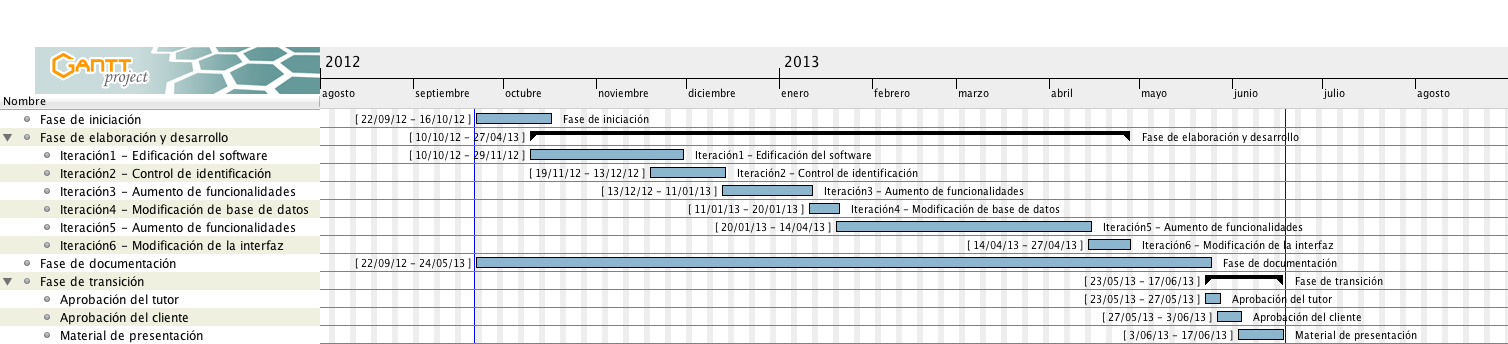
\includegraphics[totalheight=6cm,width=16cm]{gantt}
  \caption{Diagrama de Gantt}
  \label{gannt}
\end{figure}

\newpage
\section{\fontsize{12}{1}\selectfont Análisis de requisitos}
\noindent En esta sección de análisis, nos centramos en lo que tiene que hacer el sistema olvidándonos de la tecnología. Para realizar el análisis de requisitos se concertaron entrevistas con el cliente, en las cuales recogimos un informe de necesidades que posteriormente formulamos como requisitos del sistema. En estas entrevistas, el cliente nos formuló cuales eran sus necesidades principales y, más tarde, en las siguientes entrevistas, llegamos a un acuerdo para que el sistema tuviese un aumento de funcionalidades y quedase más profesional. Durante estas entrevistas se estudiaron:
\renewcommand{\labelitemi}{$\diamond$}
\begin{itemize}
\item Las responsabilidades de cada tipo de actor del sistema.
\item Los requisitos funcionales que debería de tener la aplicación tales como gestión de usuarios, clientes, proveedores, productos, ventas, reservas, apartados, devoluciones, gráficas, citas e informes.
\item Los requisitos no funcionales que la aplicación debería cumplir como portabilidad, rendimiento, seguridad, interfaz de usuario y auditoría.
\end{itemize}
 En esta fase, hacemos uso de los diagramas de casos de uso para describir los pasos necesarios para cumplir un objetivo. Estudiamos los requisitos de información realizando su diagrama y, también, estudiamos el modelo de comportamiento del sistema. En la figura \ref{uml} se muestra una imagen en la que podemos apreciar el diagrama conceptual de datos del sistema.

\newpage

\begin{figure}[!ht]
  \centering
    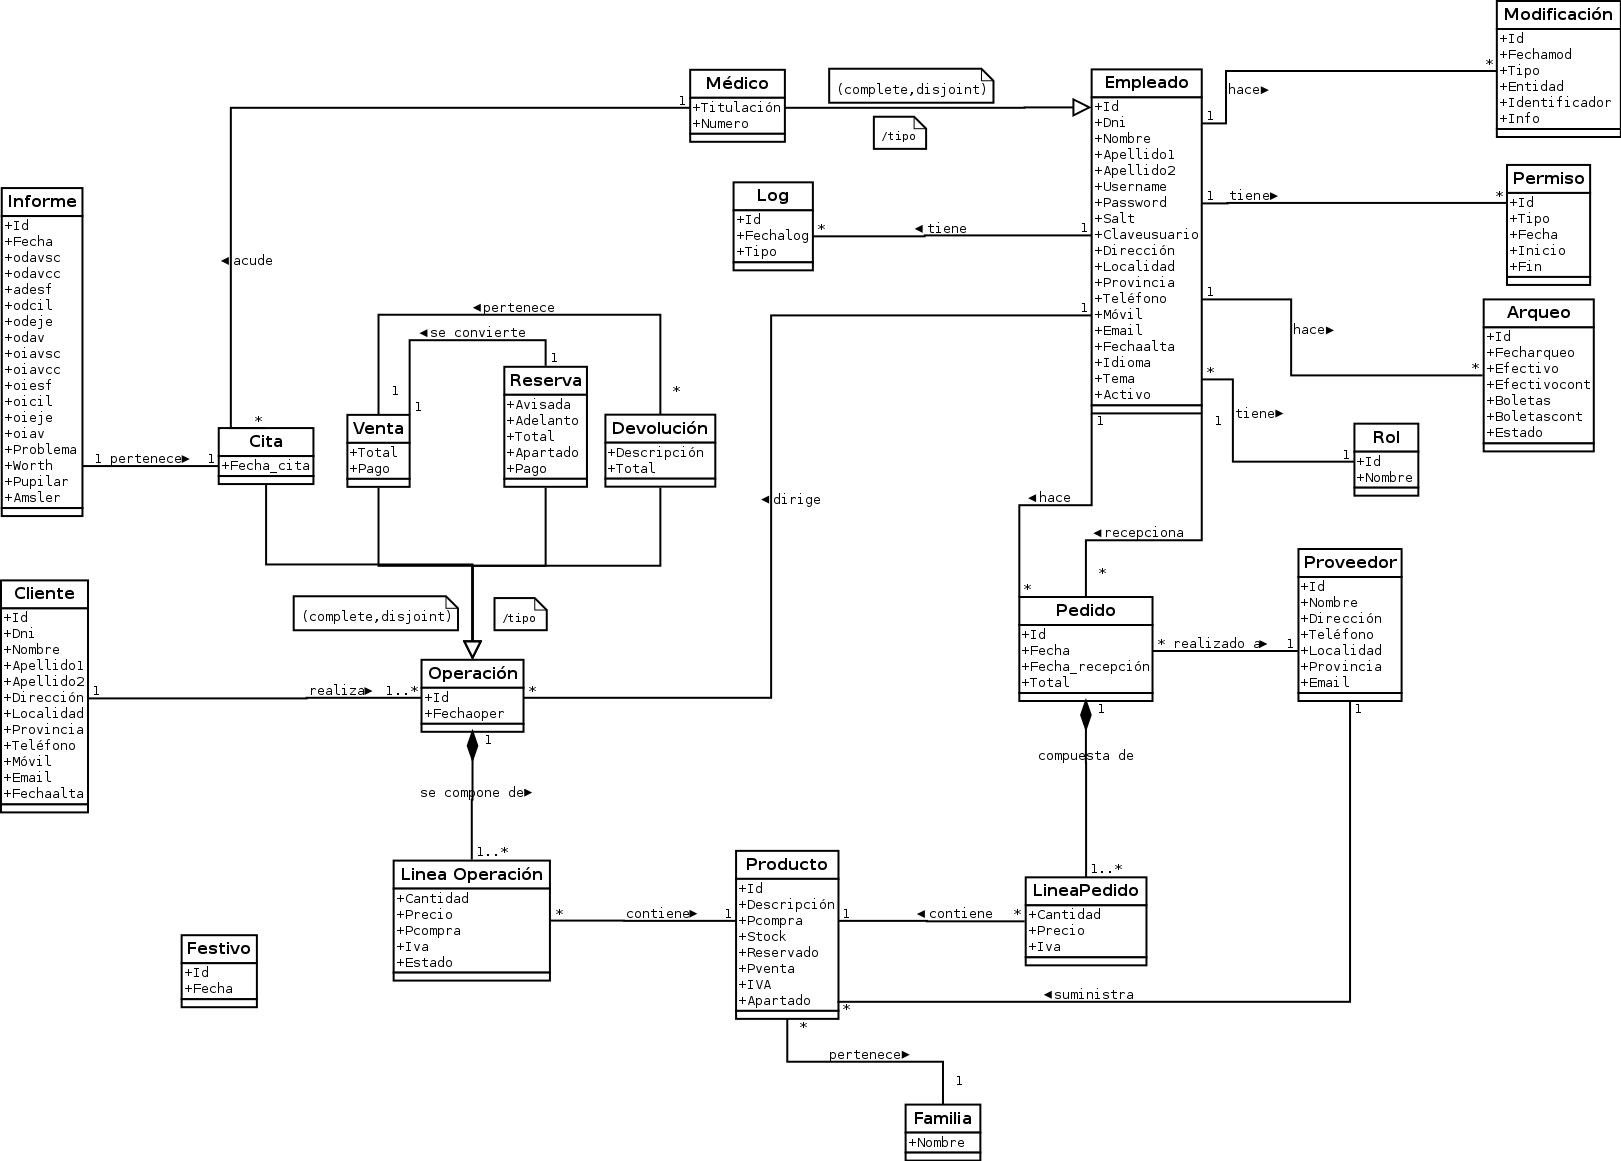
\includegraphics[angle=270,scale=0.33]{UML}
  \caption{Modelo conceptual de datos}
\label{uml}
\end{figure}

\newpage
\section{\fontsize{12}{1}\selectfont Diseño del sistema}
\noindent En el diseño del sistema nos centramos en cómo hace el sistema para cumplir los objetivos teniendo en cuenta la tecnología usada. En el diseño del sistema nos centramos en el estudio de la arquitectura general del sistema, el diseño de la interfaz de usuario y el diseño físico de componentes.\\
Para la arquitectura de la aplicación se escogió la arquitectura MVC ya que tendremos el código más organizado, sencillez para distintas representaciones y podremos reutilizar código. Esta arquitectura MVC se separa los datos y la lógica de negocio de una aplicación de la interfaz de usuario y el módulo encargado de gestionar los eventos y las comunicaciones.\\
La aplicación trabaja en un servidor web Apache con el lenguaje de programación PHP5.3+ instalado y MySQL para el banco de datos.
Para que la interfaz de usuario fuese la adecuada se hicieron prototipos que se le enseñaron al cliente el cual los aceptó. También, a medida que se iba construyendo el sistema, se le fue enseñando para que la interfaz fuese plenamente de su agrado.

\section{\fontsize{12}{1}\selectfont Implementación}

\noindent Para realizar la aplicación se ha utilizado numerosas herramientas, bibliotecas y lenguajes de programación que se describen a continuación:

\begin{itemize}
\item \textbf{Lenguajes de programación utilizados:}\\
Se ha elegido PHP como lenguaje base ya que es muy parecido al lenguaje C con una gran documentación. Para facilitarnos la tarea se ha utilizado el framework Symfony2 el cual nos aporta funciones, librerías, seguridad y velocidad entre otras cosas.
Cuando un usuario solicita una página escrita en PHP, el motor de PHP ejecuta el código y envía al usuario una página en HTML a la cual daremos un aspecto visual utilizando hojas de estilo CSS. Para dotar al sistema de interactividad se ha hecho uso del lenguaje Javascript. Para la ayuda con este lenguaje se ha usado el framework jQuery el cual nos facilita el uso del lenguaje JavaScript.

\item \textbf{Bibliotecas utilizadas:}\\
Hacemos uso de la librería de componentes jQueryUI para el framework jQuery la cual nos permite un conjunto muy amplio de widgets, plugins y efectos para usar en nuestra aplicación web.\\ Para la creación de calendarios nos ayudamos de la librería Fullcalendar, que nos proporciona poder implementar de manera muy sencilla calendarios visuales muy atractivos y fáciles de personalizar. Además, ésta permite el uso de otra librería llamada qTip para generar tooltips a los elementos del calendario.\\ Para la generación de gráficos estadísticos usamos la librería HighCharts, ya que nos permite generar distintas estadísticas interactivas dependiendo de nuestra necesidad con muy buen aspecto. \\Con respecto a las tablas que genera la aplicación, nos ayudamos de la librería Datatables la cual nos permite darle dinamismo a nuestras tablas además de conseguir la ordenación por campos, paginados, filtros, etc. \\Por último, para la generación de documentos, usamos la librería PDFBundle que nos ayuda a usar la librería FPDF dentro de un proyecto Symfony2. Los documentos se abren en una ventana modal con la ayuda de la librería de jQuery FancyBox.

\item \textbf{Herramientas utilizadas:}\\
Para poder llevar a cabo la aplicación debemos instalar LAMP que nos proporciona los elementos necesarios para un servidor web(Apache, MySQL, PHP).\\
Como editor usamos SublimeText2 ya que es muy ligero, ofrece de forma nativa infinidad de lenguajes de programación, además de poder instalar plugins como por ejemplo, LiveReload el cual nos permite ahorrarnos el trabajo de recargar la página web cuando modificamos código.\\
Para llevar un control de los archivos del proyecto usamos un software de control de versiones como GIT, ya que es ampliamente usado, gratuito y de código abierto.\\
Para la generación de los distintos documentos del proyecto hemos usado Día para la generación y edición de diagramas, Gimp para la edición de imágenes y \LaTeX{} como lenguaje de programación para la creación de documentos. Como editor de texto en \LaTeX{} hemos usado TextWorks.\\
Por último, para la generación de prototipos usamos PencilApp y GanttProject para realizar el diagrama de tiempo empleado en el proyecto.

\end{itemize}

\section{\fontsize{12}{1}\selectfont Pruebas}

\noindent Para comprobar que el sistema funcionase correctamente de acuerdo a los objetivos previamente establecidos se realizaron todo tipo de pruebas. A medida que se iba desarrollando el sistema se realizaron pruebas unitarias y de integración manuales, continuando cuando ya estaba realizada la aplicación con pruebas de sistema y de aceptación. En las pruebas de sistema comprobamos que el sistema cumple con todos los requisitos previamente establecidos tanto funcionales como no funcionales.\\
Las pruebas funcionales se realizaron manualmente comprobando que todos los escenarios, tanto principales como secundarios, funcionasen correctamente. En estas pruebas se iban comprobando los datos haciendo cálculos manuales.\\
En las pruebas no funcionales comprobamos requisitos como portabilidad, rendimiento, seguridad e interfaz de usuario. Para comprobar la seguridad se ha consultado el documento de los diez riesgos más importantes realizado por la fundación OWASP\footnote{\url{https://www.owasp.org/images/2/2d/OWASP_Top_10_-_2010_FINAL_(spanish).pdf}. \textit{OWASP}} y para la usabilidad se ha consultado la lista de los 25 puntos clave de usabilidad de UserEffect\footnote{\url{http://www.usereffect.com/download/checklist.pdf}. \textit{UserEffect}} . Para comprobar la portabilidad y el rendimiento se hicieron uso de herramientas online. En la figura \ref{gtmetrix} y \ref{pigdom} se puede ver el resultado de las pruebas de rendimiento mientras que en la figura \ref{browserstack} se puede ver el resultado de las pruebas de portabilidad.\\

\begin{figure}[!ht]
  \centering
    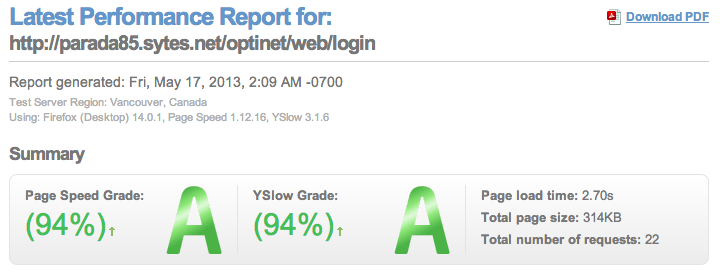
\includegraphics[scale=0.5]{ren}
  \caption{GTmetrix}
\label{gtmetrix}
\end{figure}

\begin{figure}[!ht]
  \centering
    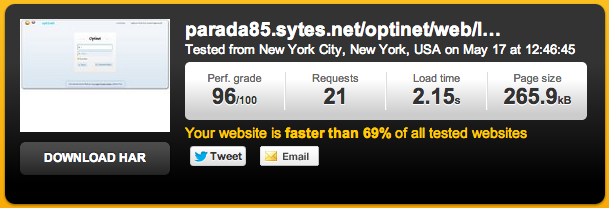
\includegraphics[scale=0.58]{renotro}
  \caption{Pigdom}
\label{pigdom}
\end{figure}

\begin{figure}[!ht]
  \centering
    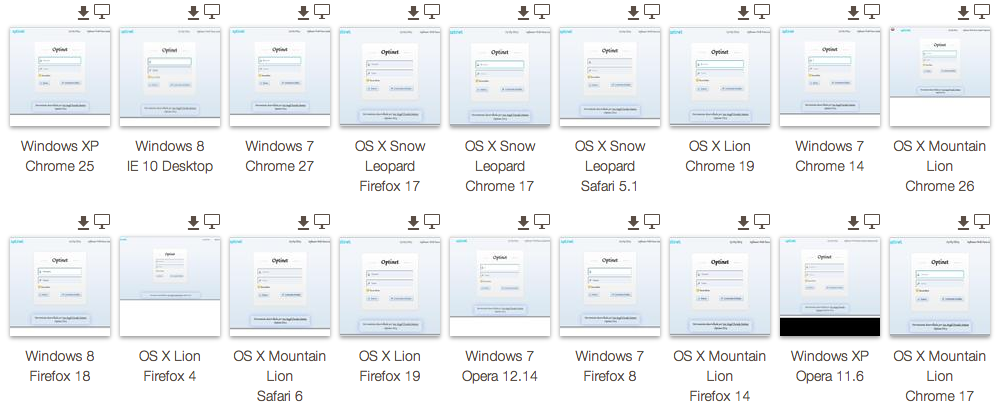
\includegraphics[scale=0.43]{browserstack}
  \caption{Browserstack}
\label{browserstack}
\end{figure}


\newpage
En las pruebas de aceptación diferenciamos a dos tipos de usuarios, por un lado usuarios con un alto nivel de conocimientos informáticos como amigos de la facultad con acceso al código y por otro lado personas con nivel bajo de conocimientos informáticos como cliente final. Los dos tipos de personas detectaron errores que fueron corregidos.

\section{\fontsize{12}{1}\selectfont Conclusiones}

\noindent La aplicación actualmente está implantada en el centro óptico y se han logrado los objetivos marcados al inicio del proyecto obteniendo así la satisfacción del cliente. A medida que se iba desarrollando el proyecto se repasaban conocimientos aprendidos durante mi formación universitaria además de ampliar y poner en práctica lenguajes de programación que serán muy valiosos de cara al futuro en el ámbito laboral. También, he aprendido a trabajar en solitario poniéndome fechas, leyendo manuales y participando en foros. A todo este trabajo en solitario se le unía la dificultad del idioma, por lo que he tenido que aprender obligatoriamente inglés técnico.\\
La aplicación se encuentra alojada en GitHub para que cualquier persona tenga acceso al código y pueda usarlo. De esta forma, aportamos nuestro granito de arena a la comunidad de software libre.

\begin{center}\url{http://github.com/parada85/optinet.git}\end{center}


\section{\fontsize{12}{1}\selectfont Bibliografía}
\begin{itemize}
\item Página oficial de Symfony. \\\url{http://www.symfony.com}
\item Manual de PHP. \\\url{http://es.php.net/manuel/es}
\item Documentación de Symfony. \\\url{http://gitnacho.github.io/symfony-docs-es}
\item Api Symfony2. \\\url{http://api.symfony.com/2.0/index.html}
\item Conferencias de Symfony2. \\\url{http://desymfony.com}
\item Libro desarrollo ágil Symfony2. \\\url{http://www.symfony.es/libro}
\item Página oficial Doctrine. \\\url{http://www.doctrine-project.org}
\item Página oficial jQuery. \\\url{http://www.jquery.com}
\item Manual jQuery. \\\url{http://librojquery.com}
\item Página oficial de jQuery Datatables. \\\url{http://www.datatables.net}
\item Página oficial de jQuery Fullcalendar. \\\url{http://arshaw.com/fullcalendar}
\item Página oficial jQuery fancybox. \\\url{http://fancybox.net}
\item Página oficial Wijmo UI. \\\url{http://wijmo.com}
\item JsRoutingBundle. \\\url{https://github.com/FriendsOfSymfony/FOSJsRoutingBundle}
\item FPDF. \\\url{http://www.fpdf.org}
\item PdfBundle. \\\url{https://github.com/psliwa/PdfBundle}
\item DoctrineFixturesBundle. \\\url{https://github.com/doctrine/DoctrineFixturesBundle}
\item Foro google Symfony2. \\\url{groups.google.es/group/symfony-es}
\item Foro programación. \\\url{http://stackoverflow.com}
\item Wikipedia RUP. \\\url{http://es.wikipedia.org/wiki/Proceso_Unificado_de_Rational}
\item El Lenguaje Unificado de Modelado. Guía de Usuario \\G. Booch, J. Rumbaugh, I. Jacobson 1999
\item UML y Patrones: Una introducción al análisis y diseño orientado a objetos y al proceso unificado \\C. Larman 2003
\end{itemize}

\section{\fontsize{12}{1}\selectfont Agradecimientos}
\noindent Para terminar el documento solo me queda agradecer a mis padres el apoyo recibido y a mi tutor del proyecto Iván Ruiz Rube por su dedicación e implicación en este proyecto. 
  
\end{document}